\section{Code Execution}\label{section:code-execution2}

As introduced in Section~\ref{section:code-execution1}, \tool utilizes Docker to run students' code in an isolated environment. This section describes the precise workflow for running a code submission.

\subsection{Workflow}

\begin{figure}
\centering
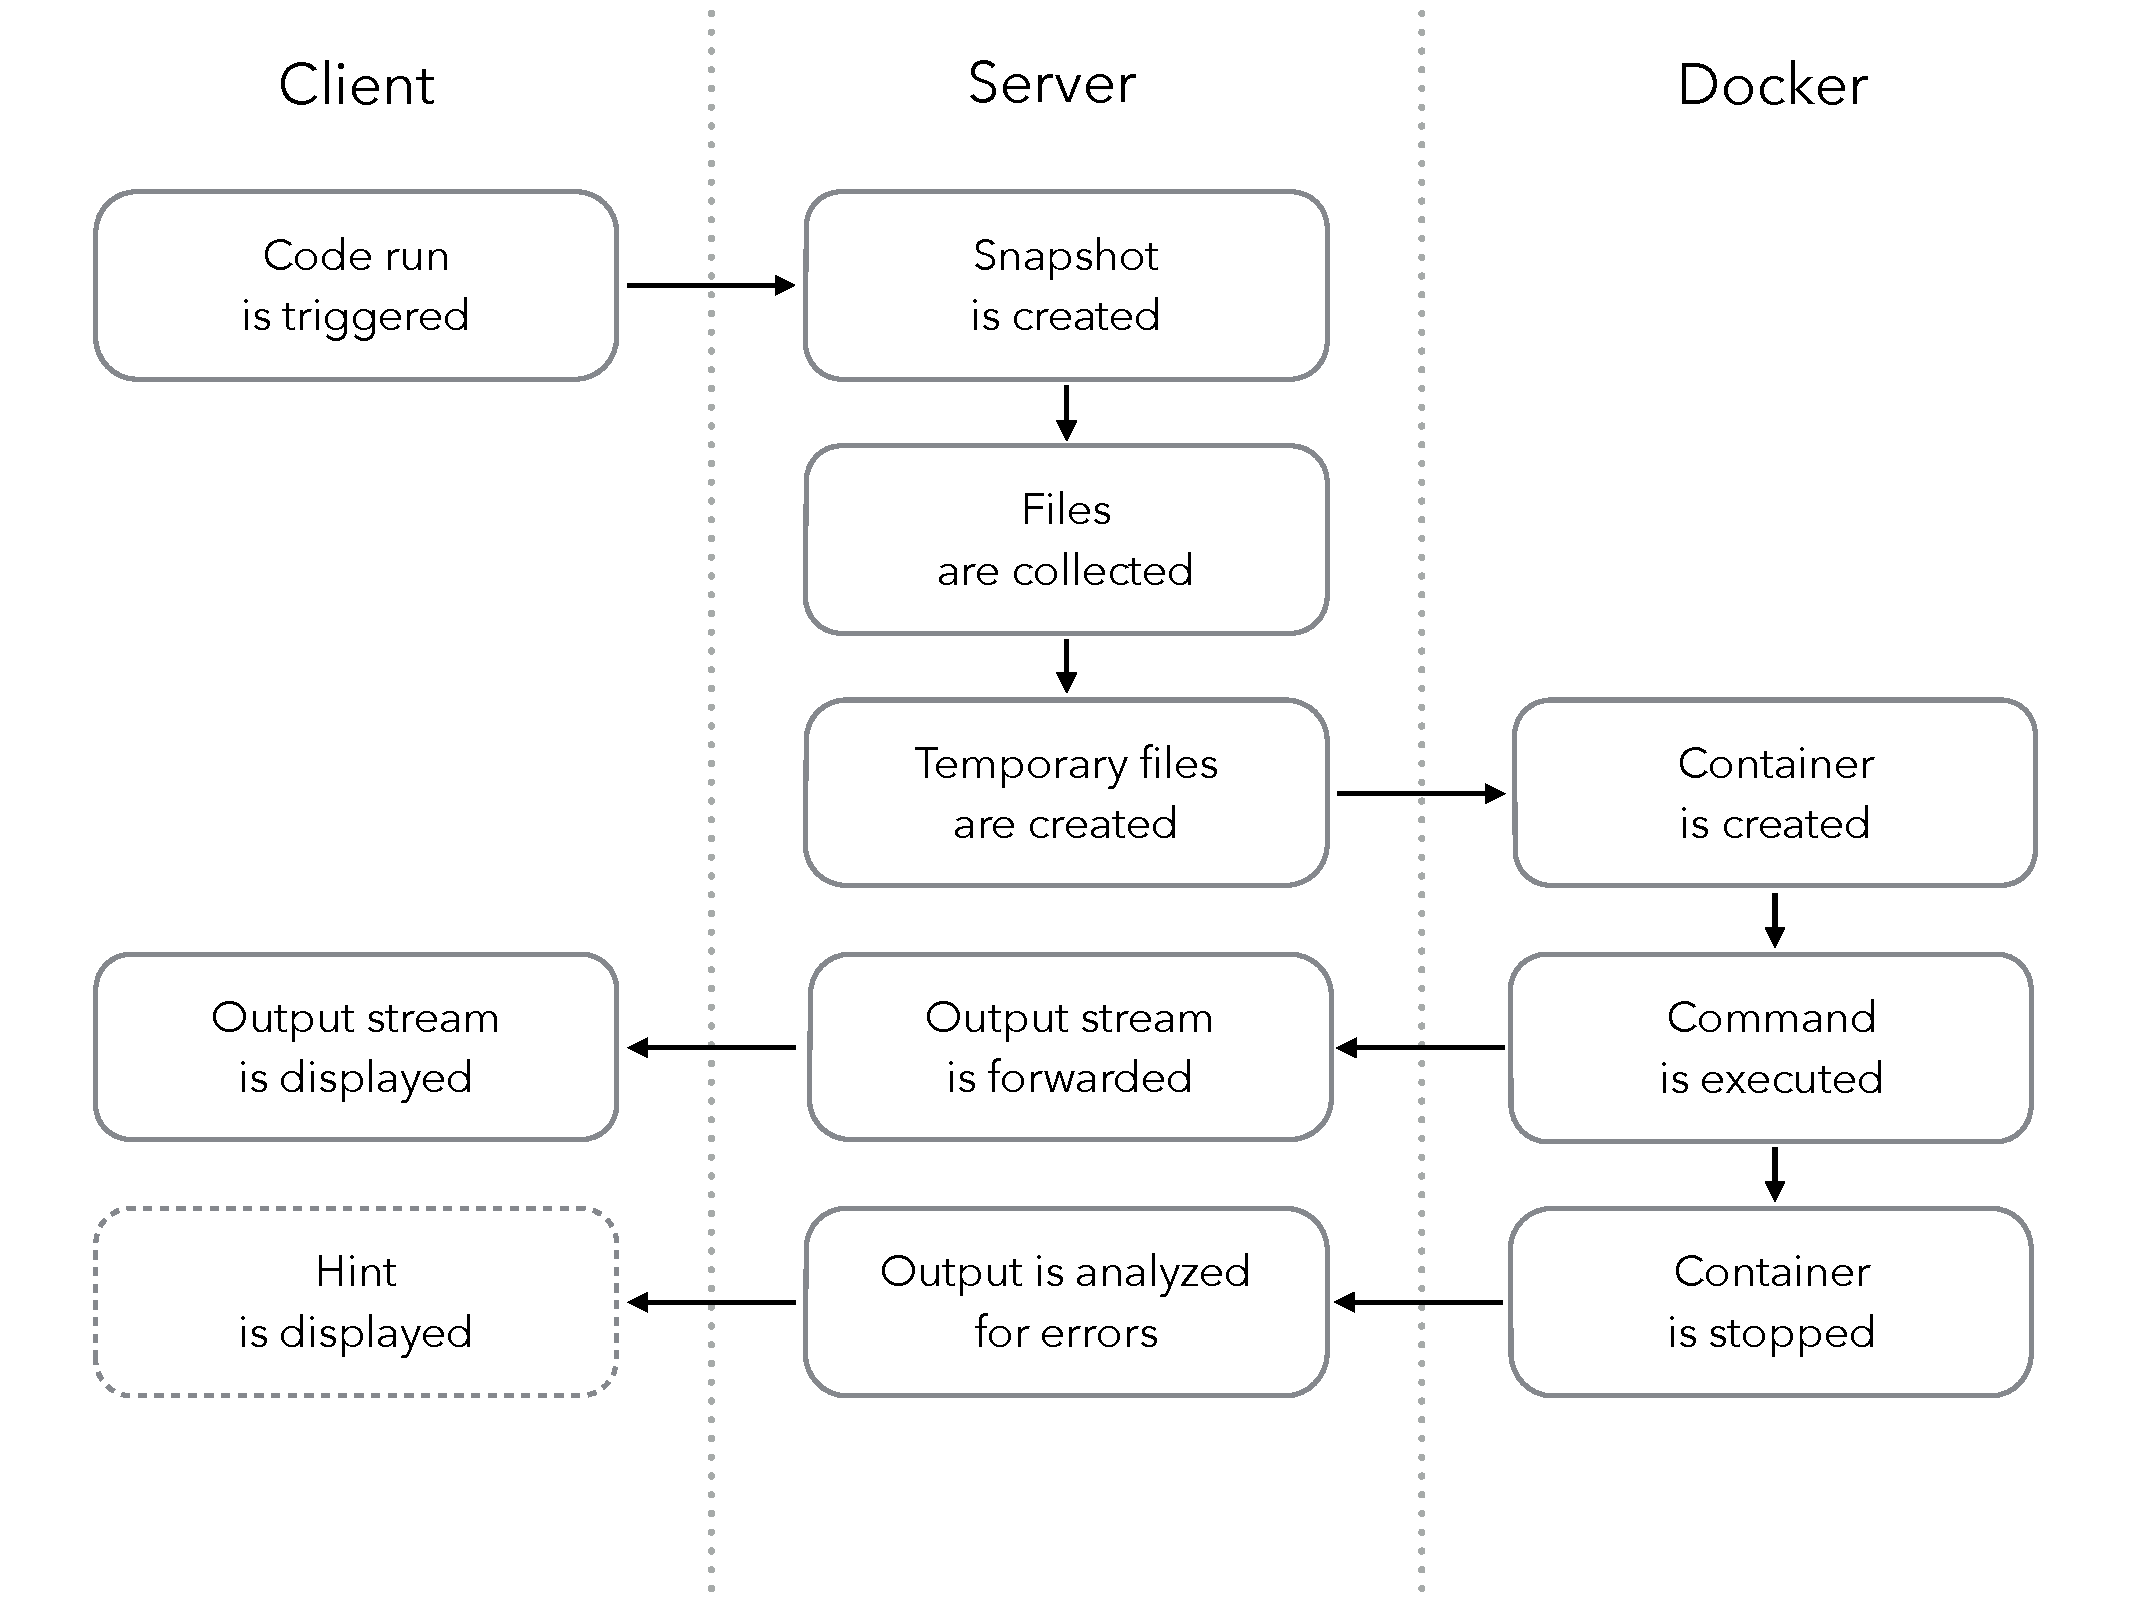
\includegraphics[clip=true, trim=0.5cm 3cm 0.5cm 0.5cm, width=\textwidth]{images/code-execution}
\caption{Code Execution Workflow}
\label{figure:code-execution}
\end{figure}

The code execution workflow involves the web application's client side, its server side, and Docker. It is depicted in Figure~\ref{figure:code-execution}.

Whenever a learner triggers a code run from the development environment, her current implementation progress is sent to the server using \gls{ajax}. A snapshot is created and stored.

To execute a code submission, a new Docker container, based on the exercise's execution environment's Docker image, is provided. Every code execution starts with a blank slate, which prevents potential side effects of previous code executions.

Based on the execution environment's configuration, a number of network ports can be exposed by the Docker container during its runtime in order to allow a student to send and receive data. To avoid port collisions among simultaneously active learners, a pool of available ports is maintained, which provides mutually exclusive access to ports.

To supply the container with the necessary files, the exercise's skeleton files plus student-written files are collected from the database and are written to a submission-specific temporary directory. Depending on the physical location of the application server in relation to the Docker server, the files can be placed in a shared folder, explicitly transferred over a network, or made available through a network or Cloud file system. In the end, the submission-specific directory is mounted as a data volume into the container's file system.

\begin{listing}
\inputminted[frame=lines]{rb}{listings/submission.rb}
\vspace{-0.33cm}
\caption{Excerpt from the \mintinline{rb}{Submission} Class Illustrating File Collection for Code Execution}
\label{listing:submission-collect-files}
\end{listing}

Listing~\ref{listing:submission-collect-files} depicts an excerpt from the \mintinline{rb}{Submission} class, which illustrates how the files needed for execution are collected. At first, all skeleton files are collected and organized according to their \glspl{id}. Subsequently, student-written files are collected and organized according to their ancestors' \glspl{id}. Finally, both collections are merged, granting priority to student-written files, which can override their ancestors.

\begin{listing}
\inputminted[frame=lines]{sh}{listings/docker-run1.sh}
\vspace{-0.33cm}
\caption{Exemplary Docker Invocation for Executing a Learner’s Code Submission}
\label{listing:docker-run1}
\end{listing}

To run a learner's submission, the execution environment's run command is executed in the prepared Docker container. Listing~\ref{listing:docker-run1} shows an exemplary invocation in Docker's \gls{cli} syntax. It specifies a shared volume mapping, the Docker image to use, and which command to execute. In this example, a Ruby-specific invocation is passed to Bash\foo{http://www.gnu.org/software/bash/}. The filename specified in the command is not hardcoded but dynamically inserted.

During execution, the Docker container's output is forwarded to the client side. After code execution has finished, the Docker container is discarded, allocated ports are released, and temporary files are deleted.

\subsection{Output Streaming}

The standard output streams of a Docker container are intercepted and supplied to the learner. Since rendering the entire output only after program execution is not sufficient for long-running processes, program output is streamed to the client in real time.

For that purpose, we decided to make use of \gls{sse}~\cite{grigorik2013high}, which is a technology that enables efficient server-to-client streaming of text-based event data using a long-lived traditional \gls{http} connection.

Since version 4, Rails offers built-in support for \gls{sse}. In this respect, Rails' \mintinline{rb}{ActionController::Live}\foo{http://api.rubyonrails.org/classes/ActionController/Live.html} module bundles functionality for real-time streaming of data to the client. In addition, the \mintinline{rb}{ActionController::Live::SSE}\foo{http://api.rubyonrails.org/classes/ActionController/Live/SSE.html} class provides the capabilities for writing events to a stream and automatically formatting the payload according to the \gls{sse} specification.

The \gls{sse} standard's client-side \gls{api} is contained in the \mintinline{js}{EventSource}\foo{http://www.w3.org/TR/eventsource/} interface that enables clients to receive push notifications from servers as \gls{dom} events. For this purpose, the client's browser maintains a connection to the server, continuously polling for new data on the response stream. Whenever the stream's data changes, an event is fired.

\Gls{sse} is available in all modern desktop browsers except Microsoft's Internet Explorer\foo{http://www.microsoft.com/download/internet-explorer.aspx}. Since \gls{sse} uses a regular \gls{http} connection, client-side functionality can be replicated entirely in JavaScript unless natively supported.

\subsection{Termination}

More often than experienced programmers, novices write non-terminating code, which can block available server processes and waste resources~\cite{loewis2014scaling}. In order to restrict the amount of wasted computing power, \tool puts a limit on Docker containers' permitted execution time. If a running container's execution time exceeds the permitted duration, for example due to an infinite loop or never-ending recursion, the container is stopped and the learner is notified that she has built a non-terminating program.

Besides cutting down infinite loops, limiting execution time can also be used as a measure of quality assessment since an efficiency limit for code submissions can be enforced~\cite{pieterse2013automated}.

The permitted execution time of an execution environment can be tailored to the needs of a certain course. A few seconds of execution time should be enough for simple programs developed in a beginners' course, while wasted execution time is limited efficiently. A longer execution time should be granted to advanced courses involving intentionally long-running programs, complex \gls{sql} queries, or heavy computations.
